\documentclass[11pt,a4paper]{article}
\usepackage[utf8]{inputenc}
\usepackage[T1]{fontenc}
\usepackage{mathptmx}
\usepackage[scaled=0.92]{helvet}
\usepackage[varqu]{inconsolata}
\usepackage[a4paper,margin=2.2cm]{geometry}
\usepackage{microtype}
\usepackage{amssymb}
\usepackage{graphicx}
\usepackage{tabularx,booktabs,array}
\usepackage{float}
\usepackage{enumitem}
\usepackage{pifont}
\usepackage[dvipsnames]{xcolor}
\usepackage[font=small,labelfont=bf]{caption}
\usepackage[hidelinks]{hyperref}

\newcommand{\cmark}{\textcolor{ForestGreen}{\ding{51}}}
\newcommand{\xmark}{\textcolor{BrickRed}{\ding{55}}}
\newcommand{\code}[1]{\texttt{#1}}
\newcolumntype{Y}{>{\raggedright\arraybackslash}X}
\setlist{itemsep=2pt,topsep=3pt,parsep=0pt}
\setlength{\parskip}{4pt}
\setlength{\parindent}{0pt}
\renewcommand{\arraystretch}{1.12}

\title{Issue in, reviewed PR out:\\ an agentic SDLC workflow for tinydb}
\author{AutoSE Assignment 3 \quad Roll number 2023111028\\[2pt]
\small \url{https://github.com/Harshit-Lalwani/AutoSE-A3-tinydb}}
\date{}

\begin{document}
\maketitle
\vspace{-1.5em}

\noindent The repository is a fork of tinydb pinned at \code{edff96a}. Every run, pull request and review cited
below is linked in \code{results/runs.md}; per-run numbers are in \code{results/results.csv}.

%======================================================================
\section{Architecture}

\begin{itemize}
  \item A maintainer adds the label \code{autose} or comments \code{/autose} on an issue. A gate job checks
        that the user has write access.
  \item A Python state machine runs four narrow LLM agents: spec, design, coder and tester. Every hand-off
        between them is decided by a deterministic check.
  \item Non-LLM code pushes the branch, opens the PR and runs CI.
  \item A reviewer from a different model family reviews the PR in a separate job with read-only access.
        Requested changes go back to design or implementation at most twice. A person merges or closes;
        the workflow never merges.
  \item Agents never see a GitHub token or an API key.
\end{itemize}

\begin{figure}[H]
  \centering
  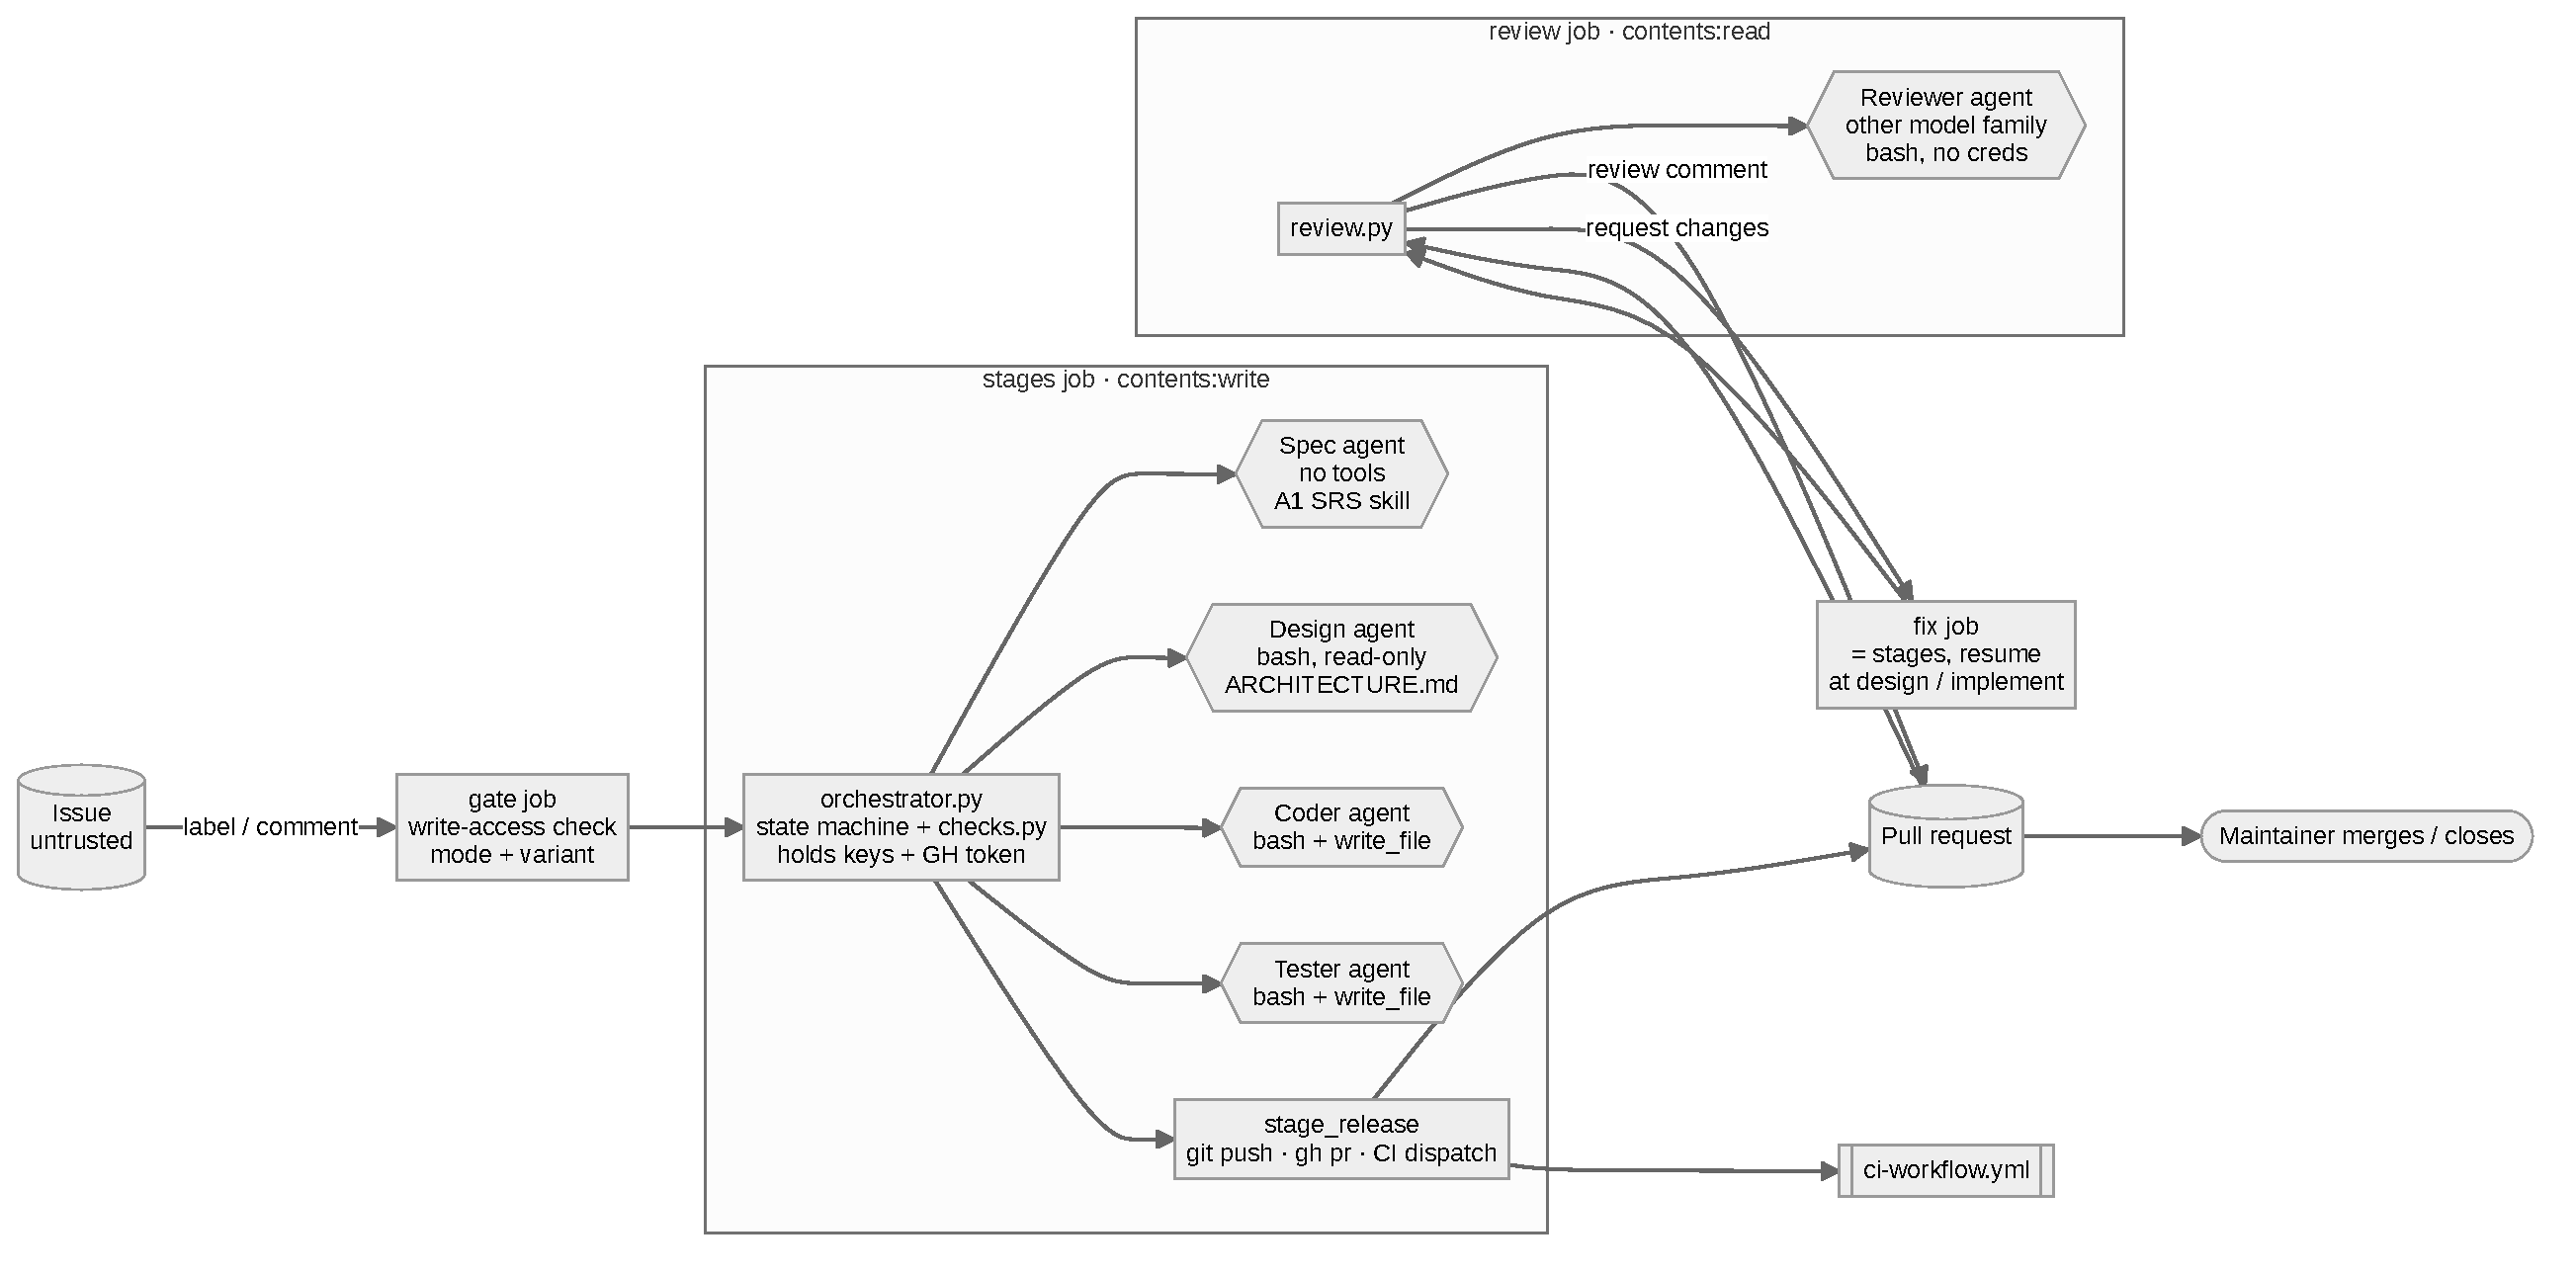
\includegraphics[width=\linewidth]{fig/component.pdf}
  \caption{Component view. Hexagons are LLM agents (Nemotron-3 Ultra builders, MiniMax M3.1 Flash reviewer,
  ADR-011). Agent commands run as a separate Unix user \code{agent} with an empty environment (ADR-005).}
\end{figure}

\begin{table}[H]
\centering\small
\begin{tabularx}{\linewidth}{@{}l l l Y Y@{}}
\toprule
\textbf{Stage} & \textbf{Agent} & \textbf{Artifact} & \textbf{Check (decided by code)} & \textbf{On failure} \\
\midrule
1 Requirements & Spec (A1 SRS skill) & \code{spec.md} & every AC in Given/When/Then, no vague words, no blocking question & 1 retry, then ask on the issue \\
2 Design & Design & \code{design.md} & planned files exist and name the functions to change & 1 retry, stop \\
3 Implementation & Coder & \code{diff.patch} & diff only in planned files or tests; AST, import, \code{mypy} & 3 attempts shared with 4 \\
4 Testing & Tester & \code{test\_report.md} & one \code{test\_ac<k>\_*} per AC; suite green; mypy; $\geq$1 new test fails on \code{main} & back to 3; re-design once \\
5 Release & none (code) & PR & PR open, CI on the PR head green & stop \\
6 Review & Reviewer & \code{review.md} & valid verdict; \code{approve} only with commands run & back to 2 or 3, max.\ 2 \\
\bottomrule
\end{tabularx}
\caption{Stage map.}
\end{table}

\begin{figure}[H]
  \centering
  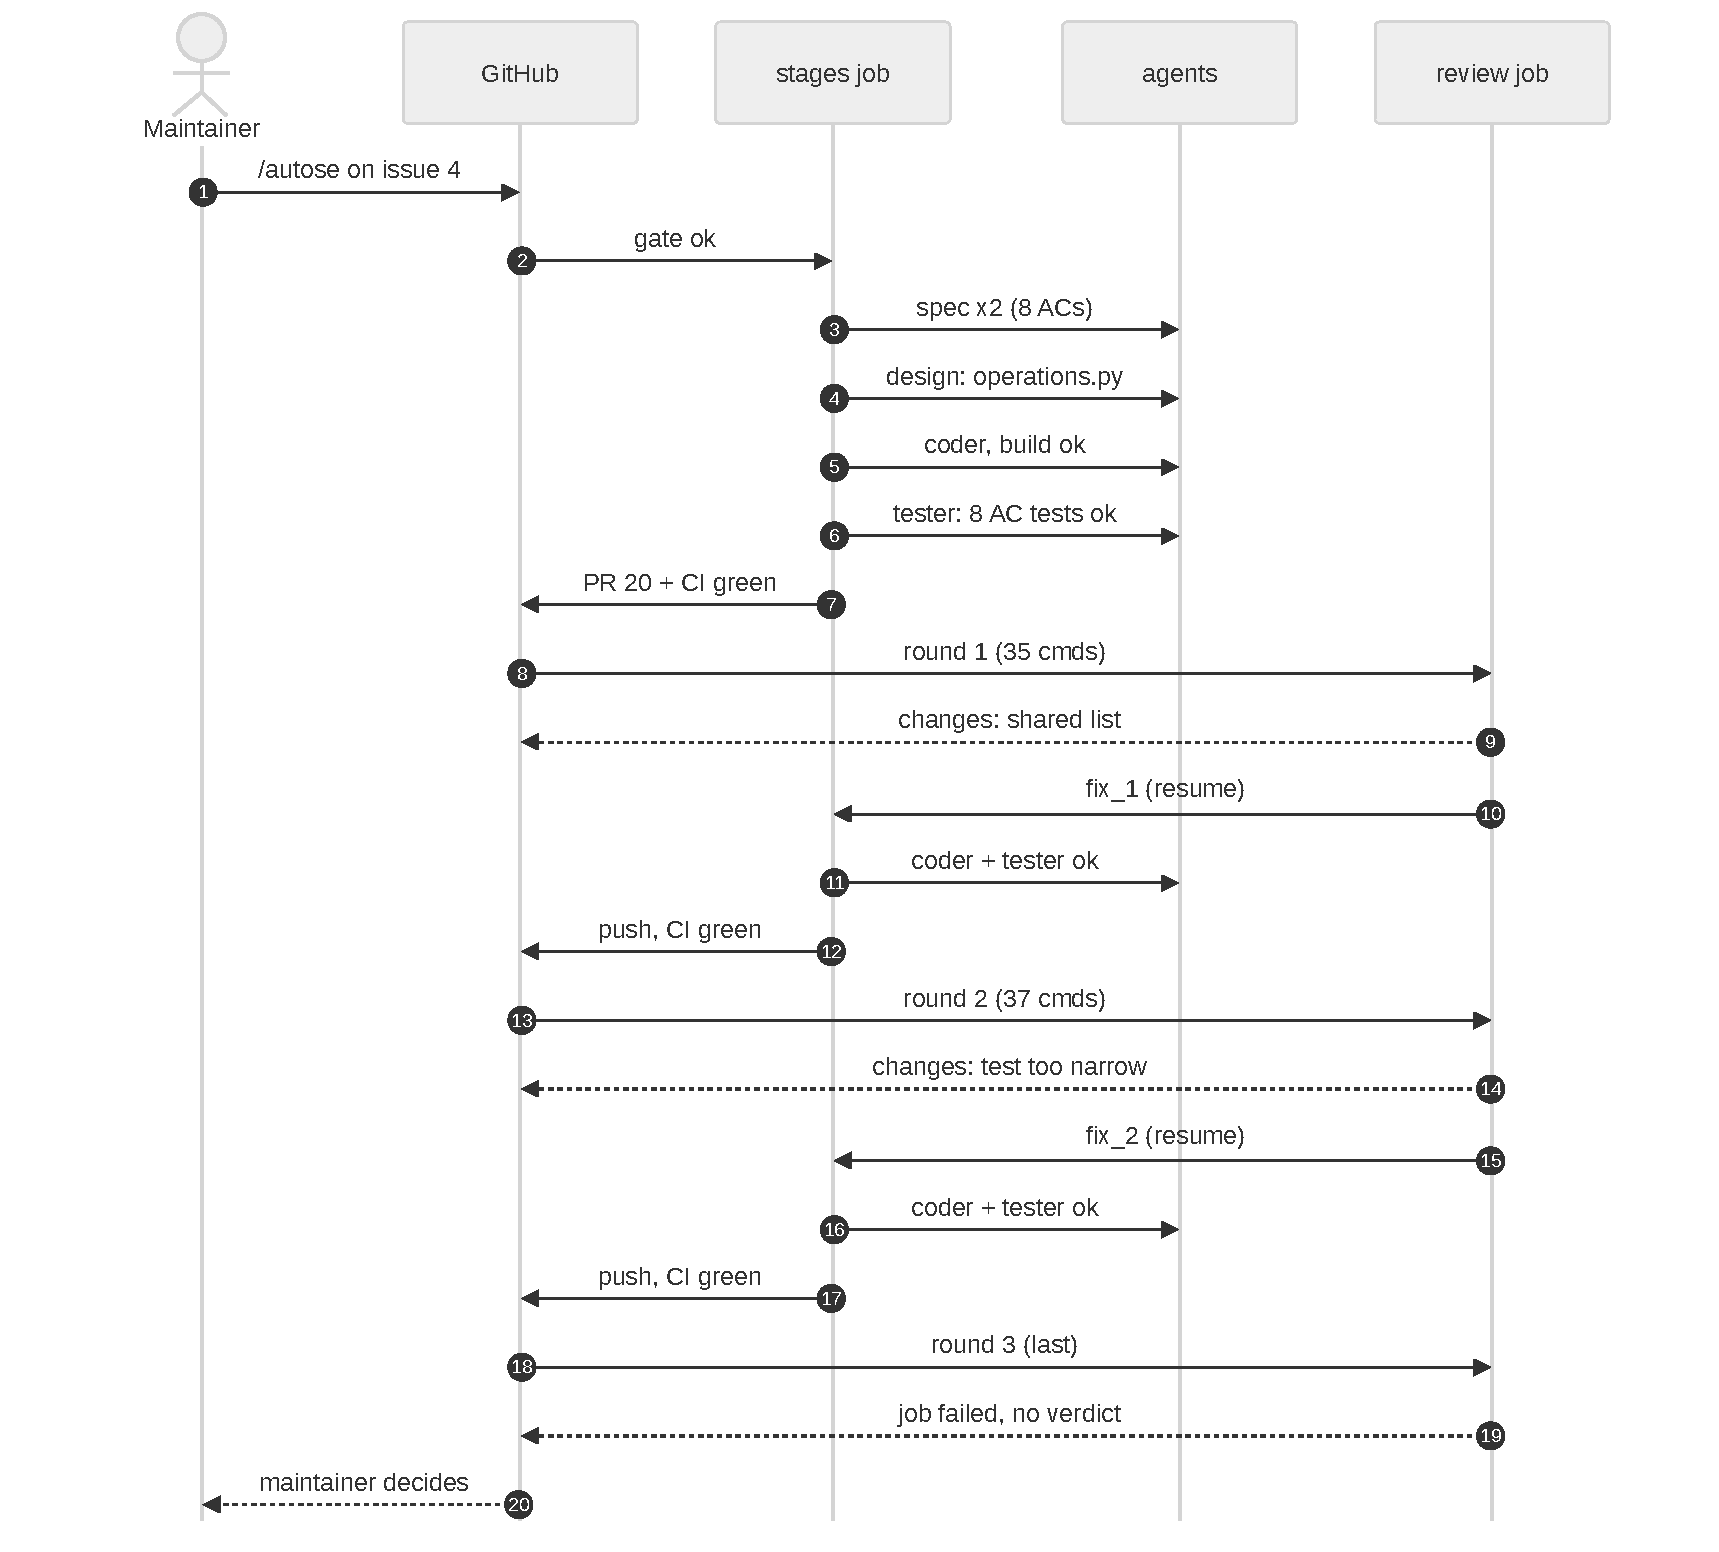
\includegraphics[width=0.6\linewidth]{fig/sequence.pdf}
  \caption{Sequence view of one real run: issue \#4 (append operation), run 45454368595, PR \#20.}
\end{figure}

\paragraph{The run in the sequence view.}
\begin{itemize}
  \item The spec agent's first answer had three blocking questions; the retry gave 8 testable acceptance
        criteria. Design, coder and tester then passed on the first attempt and PR \#20 was opened with
        green CI.
  \item Review round 1 found that \code{append} mutated a list shared by two documents (I reproduced it).
        Round 2 found a test that only holds for \code{MemoryStorage}, and unrelated files in the PR. The
        second finding was a workflow bug: fix rounds compared against the newest \code{main} (fixed in PR \#26).
  \item Round 3 failed without a verdict because the GitHub runner lost its connection. The builders used 2.32\,M of
        the 2.5\,M token budget.
\end{itemize}

%======================================================================
\section{Design decisions}

\begin{table}[H]
\centering\footnotesize
\begin{tabularx}{\linewidth}{@{}l l Y Y Y l@{}}
\toprule
\textbf{ADR} & \textbf{Area} & \textbf{Chosen} & \textbf{Main rejected option} & \textbf{Main reason} & \textbf{Status} \\
\midrule
001 & D1 Splitting & 4 narrow agents, code release, reviewer & one agent for everything & the author of the code should not write the tests that judge it & Accepted (E2) \\
002 & D2 Control & code state machine; review rounds as chained jobs & LLM planner & the graph is known; a planner can skip checks & Accepted \\
003 & D3 Hand-offs & checked artifacts; issue text only reaches the spec agent & full transcripts & keeps injected text and old mistakes out & Accepted \\
004 & D4 State & Actions artifacts and the branch & artifacts on the branch & the reviewer must not see them & Accepted \\
005 & D5 Tools & own loop, \code{bash} + \code{write\_file}, sandbox user & GitHub MCP for agents & agents never need GitHub & Accepted \\
006 & D6 Models & MiniMax builders, Nemotron reviewer & -- & one-token ping test & Superseded by 011 \\
007 & D7 Checks & deterministic check per stage & LLM judge per stage & a judge can be argued into a pass & Superseded by 013 \\
008 & D8 Reviewer & own job, inputs, model, prompt; approvals need evidence & reviewer sees PR description & anchoring on the implementer & Accepted (E1) \\
009 & D9 Safety & budgets at 3 levels; issue text as data & prompt-only defence & works even if detection fails & Accepted \\
010 & D10 Triggers & label or \code{/autose} from writers; one queue per issue & every new issue & cost; races on one branch & Accepted \\
011 & D6 Models & Nemotron-3 Ultra builders, MiniMax reviewer (no thinking) & MiniMax with reasoning & 110--238\,s per call, empty answers & Accepted \\
012 & D9 Cost & token budget: 2.5\,M per run, 400\,k per review & dollar limit & free tiers have none & Accepted \\
013 & D7 Checks & unknown function names count as new & ``symbol must exist'' & 3 of 4 first runs stopped on valid plans & Accepted \\
014 & D4/D9 Context & agents see only their last 4 tool exchanges in full & raise the budget & 6 of 7 default runs ran out of budget & Accepted \\
\bottomrule
\end{tabularx}
\caption{All ADRs. Full records, including the superseded ones, are in \code{architecture/decisions/}.}
\end{table}

The three decisions that mattered most:

\subsection{Code decides every hand-off (ADR-002, ADR-007, ADR-013)}
\begin{itemize}
  \item Every transition depends on a deterministic check, never on what a model says about its own
        work. Retries are also in code: 3 implementation attempts, one re-design, at most two review rounds.
  \item The test stage has the strongest checks: one test per acceptance criterion, the full suite, mypy on
        the new tests, and at least one new test that fails on \code{main}, so empty tests cannot pass.
  \item I rejected an LLM planner and per-stage LLM judges: a planner can skip a check, and a judge can be
        talked into a pass by the agent it judges.
  \item Result: every failed run stopped at a named check, with the reason posted on the issue.
  \item Cost: ADR-007's design check required every named function to exist already, and three of the
        first four runs stopped on correct plans that named a new function. ADR-013 replaced it. A check
        should reject wrong work, not a broken format convention.
\end{itemize}

\subsection{Least privilege enforced by the OS (ADR-005, with ADR-003 and ADR-009)}
\begin{itemize}
  \item Agents get two tools, \code{bash} and \code{write\_file}, from a small loop of my own (about 200
        lines). No agent needs GitHub: pushing, the PR and CI are done by code.
  \item Tool commands run as a separate Unix user with an empty environment, in a copy of the repository,
        so the keys held by the orchestrator cannot be read even by an agent that tries.
  \item Only the spec agent sees the raw issue text, and it has no tools. The design agent's changes are
        reset; the coder cannot change the tests and the tester cannot change the source.
  \item Rejected: the GitHub MCP server with a scoped token. It is simpler, but it turns prompt injection
        into write access to the repository.
\end{itemize}

\subsection{An independent reviewer that must show evidence (ADR-008)}
\begin{itemize}
  \item The reviewer runs in its own job with read-only access, sees only the issue, the diff and the
        repository, and uses a different model family with an adversarial prompt.
  \item Code turns an \code{approve} without any command run into \code{request\_changes}.
  \item Rejected: giving it the PR description and design for context, which I expected to anchor it on
        the implementer's claims. Experiment E1 tests this.
\end{itemize}

\paragraph{Superseded decisions.} ADR-006 chose models with a one-token ping. On real prompts MiniMax with
reasoning took 110--238\,s per call and sometimes returned nothing, so ADR-011 chose models from
measurements. ADR-007 was replaced as described above.

%======================================================================
\section{Decision experiments}

Each experiment changes one decision and keeps models, prompts, checks and budgets fixed
(\nolinkurl{experiment/variants.md}). The hypotheses were written before the runs.

\subsection{E1: reviewer isolation (ADR-008)}
\begin{itemize}
  \item \textbf{Variant.} The \emph{informed} reviewer also sees the PR description and \code{design.md}.
        The \emph{isolated} baseline sees only the issue, the diff and the repository.
  \item \textbf{Setup.} Five seeded PRs, each reviewed once by each variant.
  \item \textbf{Hypothesis.} The informed reviewer approves more, especially S3 (a band-aid whose
        description argues that it fixes the bug) and S4 (scope creep next to a correct feature).
\end{itemize}

\begin{table}[H]
\centering\small
\begin{tabularx}{\linewidth}{@{}l Y Y Y@{}}
\toprule
\textbf{PR} & \textbf{Ground truth} & \textbf{Isolated} & \textbf{Informed} \\
\midrule
S1 (\#6) & exclusive upper bound & \cmark{} request changes & \cmark{} request changes \\
S2 (\#7) & unknown string IDs raise (found by the reviewer) & \cmark{} request changes & \cmark{} request changes \\
S3 (\#8) & only clears the cache & \cmark{} request changes & \cmark{} request changes \\
S4 (\#9) & \code{delete()} silently changed & \xmark{} approve (change noted as minor) & \cmark{} request changes (major) \\
S5 (\#10) & correct & \cmark{} approve & \cmark{} approve \\
\midrule
mean & & 205\,k tokens, 25.6 commands & 215\,k tokens, 29.0 commands \\
\bottomrule
\end{tabularx}
\caption{E1 verdicts. Both variants named the same defect in S1--S3.}
\end{table}

\begin{itemize}
  \item S2 was meant to be correct. The reviewer showed that non-numeric string IDs now raise
        \code{ValueError} instead of being skipped, as the issue asks. I reproduced it, so S2 counts as defective
        (noted in \code{labels.csv}; the original label is kept).
  \item \textbf{Result: the hypothesis did not hold.} The isolated reviewer sent back 3 of 4 defective PRs,
        the informed one 4 of 4. Neither flagged the correct PR. S3's description did not talk the informed
        reviewer into an approval.
  \item The only difference went the other way. Both reviewers noticed the \code{delete()} change in S4; the
        isolated one called it minor and approved, the informed one quoted the PR description's own mention of
        the change and the project's rule on breaking changes, and asked for changes.
  \item \textbf{What I changed.} Nothing in the information split. The S4 miss is a decision-rule problem:
        the reviewer approved next to a finding it said ``should be reverted''.
\end{itemize}

\subsection{E2: separate tester or not (ADR-001)}
\begin{itemize}
  \item \textbf{Variant.} \emph{Single}: the coder writes the code and the acceptance tests, with no tester.
        \emph{Default}: a separate tester with a fresh context writes the tests. The same checks apply to both.
  \item \textbf{Setup.} Issues \#1--\#4, all runs since ADR-013.
  \item \textbf{Hypothesis.} The separate tester writes stronger tests and catches more coder mistakes, at
        a higher token cost.
\end{itemize}

\begin{table}[H]
\centering\small
\begin{tabularx}{\linewidth}{@{}l Y Y@{}}
\toprule
 & \textbf{Default (separate tester)} & \textbf{Single (coder writes tests)} \\
\midrule
runs & 9 & 6 \\
opened a PR & 2, both for \#4 (PR \#20) & 4, one per issue (PRs \#15, \#17, \#23, \#24) \\
stopped by & token budget 4, build 2, design 1 & token budget 1, design 1 \\
CI on the PR & 2 green & 1 green; 2 red from a CI bug (\#18); 1 red from its own flaky test \\
hidden tests & 4/4 & 16/16 \\
review & \#20: changes requested twice & \#15 approved; \#17, \#24 changes requested \\
builder tokens (median) & 1.68\,M & 0.73\,M \\
\bottomrule
\end{tabularx}
\caption{E2 results.}
\end{table}

\begin{itemize}
  \item \textbf{Result: the hypothesis did not hold.} The single variant opened a PR for every issue and
        passed every hidden test; the default variant did so in 2 of 9 runs.
  \item The cost came from what the split triggered. The tester re-explores the code in a fresh context (up
        to 470\,k tokens in one call), its failures send the coder back with a long pytest log, and each round
        re-sent the whole history. Most default runs ran out of budget in the implement--test loop.
  \item The single variant's weaknesses showed up later: its own wall-clock test was flaky and failed CI on
        PR \#23, and the reviewer found defects in \#17 and \#24 that no test covered.
  \item \textbf{What I changed.} I kept the separate tester, since a flaky self-written test is what it is
        there to catch, and fixed the cost instead: ADR-014 keeps only the last four tool exchanges in full,
        and agents answer before the budget runs out. After that, default runs stayed under budget (about
        1.5\,M tokens) but failed for another reason (Section~\ref{sec:hindsight}).
\end{itemize}

%======================================================================
\section{Results}

\begin{table}[H]
\centering\small
\begin{tabular}{@{}l rrr rrr@{}}
\toprule
 & \multicolumn{3}{c}{\textbf{Default (17 runs)}} & \multicolumn{3}{c}{\textbf{Single (6 runs)}} \\
\cmidrule(lr){2-4}\cmidrule(lr){5-7}
\textbf{Stage} & entered & passed & 1st try & entered & passed & 1st try \\
\midrule
1 Spec & 17 & 16 & 0 & 6 & 6 & 0 \\
2 Design & 16 & 13 & 11 & 6 & 5 & 5 \\
3 Implement & 13 & 10 & 7 & 5 & 4 & 4 \\
4 Test & 10 & 3 & 3 & 4 & 4 & 4 \\
5 Release (PR + CI) & 3 & 3 & 3 & 4 & 1 & 1 \\
6 Review (verdict posted) & 3 & 2 & -- & 4 & 3 & -- \\
\bottomrule
\end{tabular}
\caption{Pass rate per stage over the 23 pipeline runs (\code{stage\_rates.py}). A stage passes if any attempt passed; fix rounds are not counted.}
\end{table}

\begin{itemize}
  \item \textbf{Spec} never passed on the first try: every first answer, also on clear issues, listed
        blocking questions, and the retry turned most of them into stated assumptions.
  \item \textbf{Design} failures came from the old strict symbol check and from the model writing a tool
        call or a file instead of the plan (fixed in ADR-013 and its addenda).
  \item \textbf{Test} is where the default variant lost: 3 of 10 runs passed. The rest ran out of budget or
        broke the build in the implement--test loop.
  \item \textbf{Release} failed only on CI: twice from a CI bug, once on a flaky test.
  \item \textbf{Hidden tests.} All six PRs passed all their hidden tests (24/24). No run opened a PR for the
        vague issue \#5: one run stopped at the spec stage and asked the maintainer a question, which is the
        intended outcome; the other three assumed an API and stopped later.
\end{itemize}

\begin{table}[H]
\centering\small
\begin{tabularx}{\linewidth}{@{}l l Y@{}}
\toprule
\textbf{PR} & \textbf{Verdict} & \textbf{Finding (each one reproduced by hand)} \\
\midrule
S1, S2, S3 & changes (both variants) & the planted defects, plus the unplanted one in S2 \\
\#17 (single) & changes & the fix does not hold under \code{CachingMiddleware} \\
\#24 (single) & changes & \code{remove(doc\_ids=[1.5])} deletes document 1 \\
\#20 round 1 & changes & \code{append} mutates a list shared by two documents \\
\#20 round 2 & changes & test only holds for \code{MemoryStorage}; unrelated files (workflow bug) \\
\#14, \#15 & approve & minor notes only \\
\bottomrule
\end{tabularx}
\caption{What the reviewer caught (16 reviews with a verdict).}
\end{table}

\begin{itemize}
  \item \textbf{The reviewer was stronger than the hidden tests.} The hidden tests passed on PRs \#17, \#24
        and \#20 while the reviewer found the defects above.
  \item \textbf{Where it was wrong.} One false approval (S4, isolated) and one overstated finding (on \#17
        it rated ``deep copy fails for non-copyable values'' as major, although tinydb stores JSON data). No
        false alarm on the correct PR.
  \item Two reviews stopped without a verdict when the review budget ran out (fixed afterwards), and seven
        review jobs were lost to timeouts or rate limits.
  \item \textbf{Cost.} 37.8\,M tokens over all GitHub runs (32.9\,M builders, 4.9\,M reviewer), not counting
        jobs that left no artifacts or local development runs. All models were free tier.
\end{itemize}

%======================================================================
\section{Hindsight}\label{sec:hindsight}

I would change the tool set of ADR-005 first.
\begin{itemize}
  \item Tool output is cut to its first and last 4\,k characters, and \code{write\_file} replaces a whole
        file. In run 45463731962 the coder read the 30\,k-character \code{table.py}, saw the middle cut out,
        rewrote the whole file from that view and broke the build three times.
  \item The loop also re-sent every old output and file write, so cost grew with the square of the number
        of steps (now ADR-014).
  \item An \code{edit(path, old, new)} tool and a \code{read(path, start, end)} tool, as in mini-swe-agent
        and SWE-agent, would have avoided both. I treated ADR-005 as a security decision, but the shape of
        the tools decided most outcomes.
  \item Smaller changes: block an approval when the reviewer itself says a change should be reverted, and
        drop the spec retry prompt that argues questions away. On the vague issue it removed real questions
        in three of four runs.
\end{itemize}

%======================================================================
\section{Limitations and threats to validity}
\begin{enumerate}
  \item \textbf{Small samples.} Five issues, one or two runs per issue and variant, five seeded PRs. The same
        issue gave different outcomes in different runs, so differences between variants are anecdotes.
  \item \textbf{The workflow changed between runs.} Seven fixes were merged while runs were going. Each row
        of \code{results.csv} records the workflow commit, but the experiments still span several versions.
  \item \textbf{One author.} I wrote the issues, the hidden tests, the seeded PRs and the prompts, so the
        tests may encode my reading of an issue, and the seeded defects may be easier or harder than real ones.
  \item \textbf{Budget and load.} Most default failures were ``token budget exhausted'', so pass rates depend
        on the budget. Model latency varied about 5$\times$ with load, and five review jobs timed out for
        that reason.
  \item \textbf{Weak hidden tests.} They passed on every PR while the reviewer found three defects they miss,
        so they overstate correctness and do not separate the E2 variants.
  \item \textbf{Small target.} tinydb has one package and about 230 fast tests. A large repository would test
        the hand-offs much harder.
\end{enumerate}

\end{document}
